\includepdfset{    
    pages=-, % =- means all pages globally 
    landscape=true, 
    rotateoversize=true, 
    link=true, 
    linktodoc=true,
    pagecommand={}, % for pagenumbers
    } % global settings for \includepdf{}

\includepdf[
    nup=1x1, 
    addtotoc={
    1, subsection, 2, Angedachtes Layout der Materialkarten, ANKPrototyp
    }
]
{AKB-24-032_Prototyp_2024-02-26.pdf}

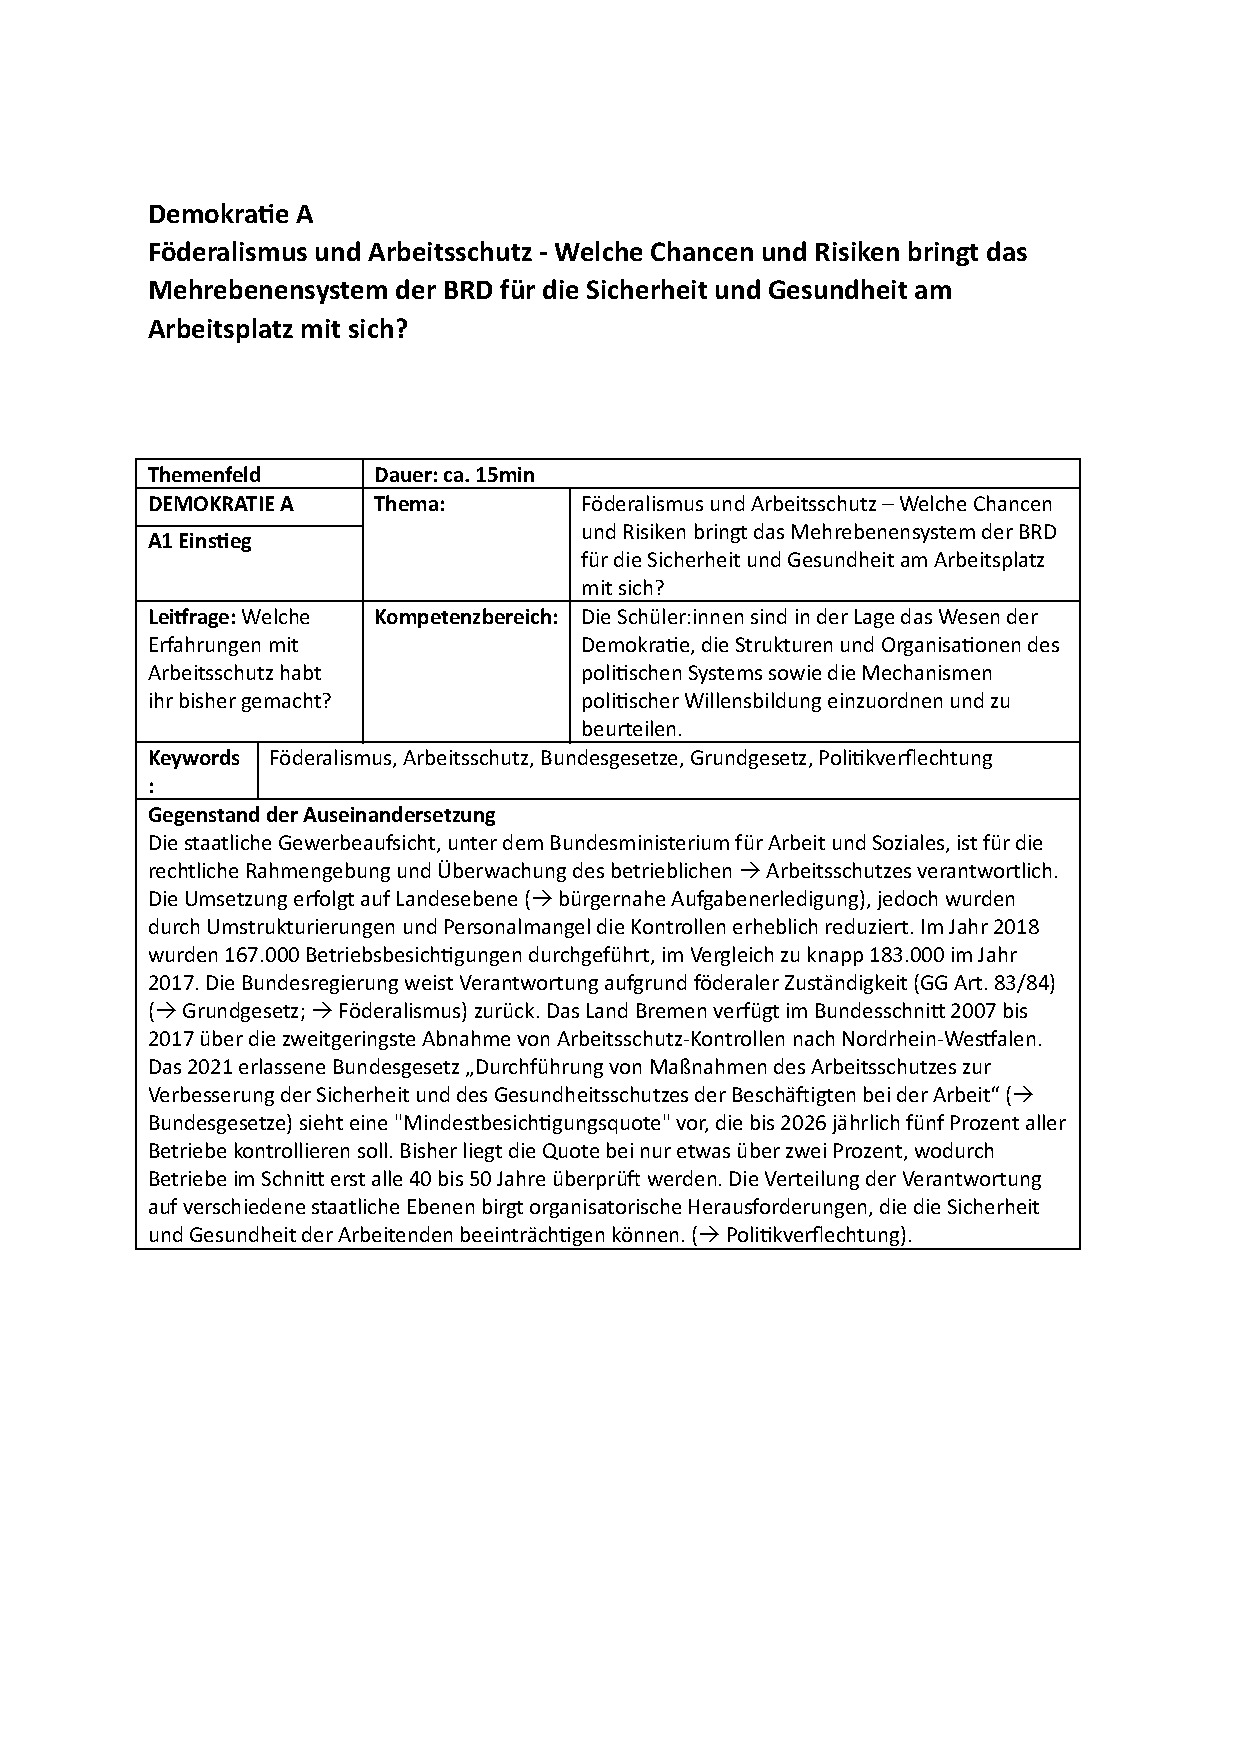
\includepdf[
    nup=2x1, 
    addtotoc={
    1, subsection, 2, Demokratie A1, DEMOKRATIE-A1, 
    3, subsection, 3, Demokratie A2, DEMOKRATIE-A2, 
    6, subsection, 2, Demokratie A3, DEMOKRATIE-A3, 
    9, subsection, 2, Demokratie B1, DEMOKRATIE-B1, 
    11, subsection, 2, Demokratie B2, DEMOKRATIE-B2, 
    13, subsection, 2, Demokratie B3, DEMOKRATIE-B3
    }
]
{DEMOKRATIE.pdf}

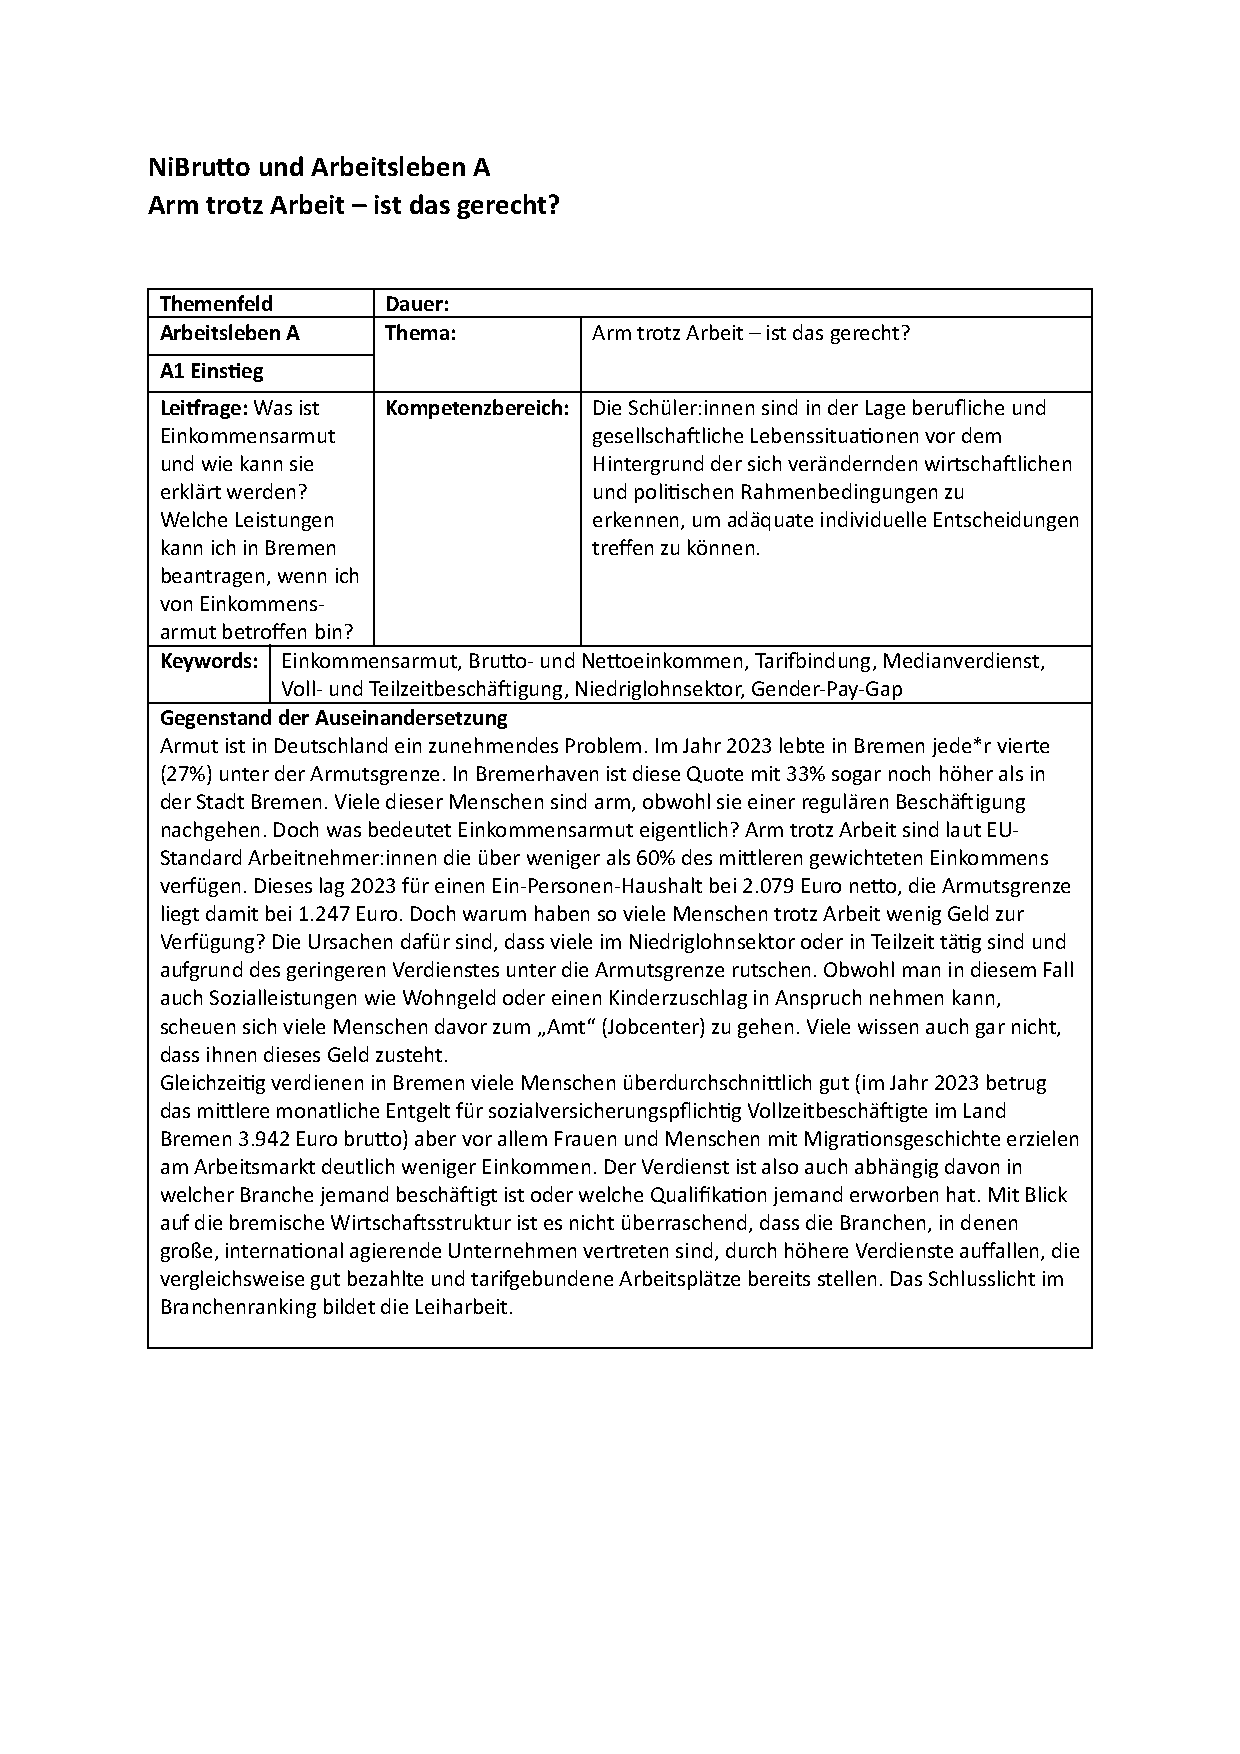
\includepdf[
    nup=2x1, 
    pages=1-14, % the last page (p. 15) is a blank box only and therefore excluded
    addtotoc={
    1, subsection, 2, Arbeitsleben A1, ARBEITSLEBEN-A1, 
    3, subsection, 2, Arbeitsleben A2, ARBEITSLEBEN-A2, 
    5, subsection, 2, Arbeitsleben B1, ARBEITSLEBEN-B1, 
    7, subsection, 2, Arbeitsleben B2, ARBEITSLEBEN-B2, 
    9, subsection, 2, Arbeitsleben B3, ARBEITSLEBEN-B3, 
    11, subsection, 2, Arbeitsleben C1, ARBEITSLEBEN-C1, 
    12, subsection, 2, Arbeitsleben C2, ARBEITSLEBEN-C2
    }
]
{ARBEITSLEBEN.pdf}

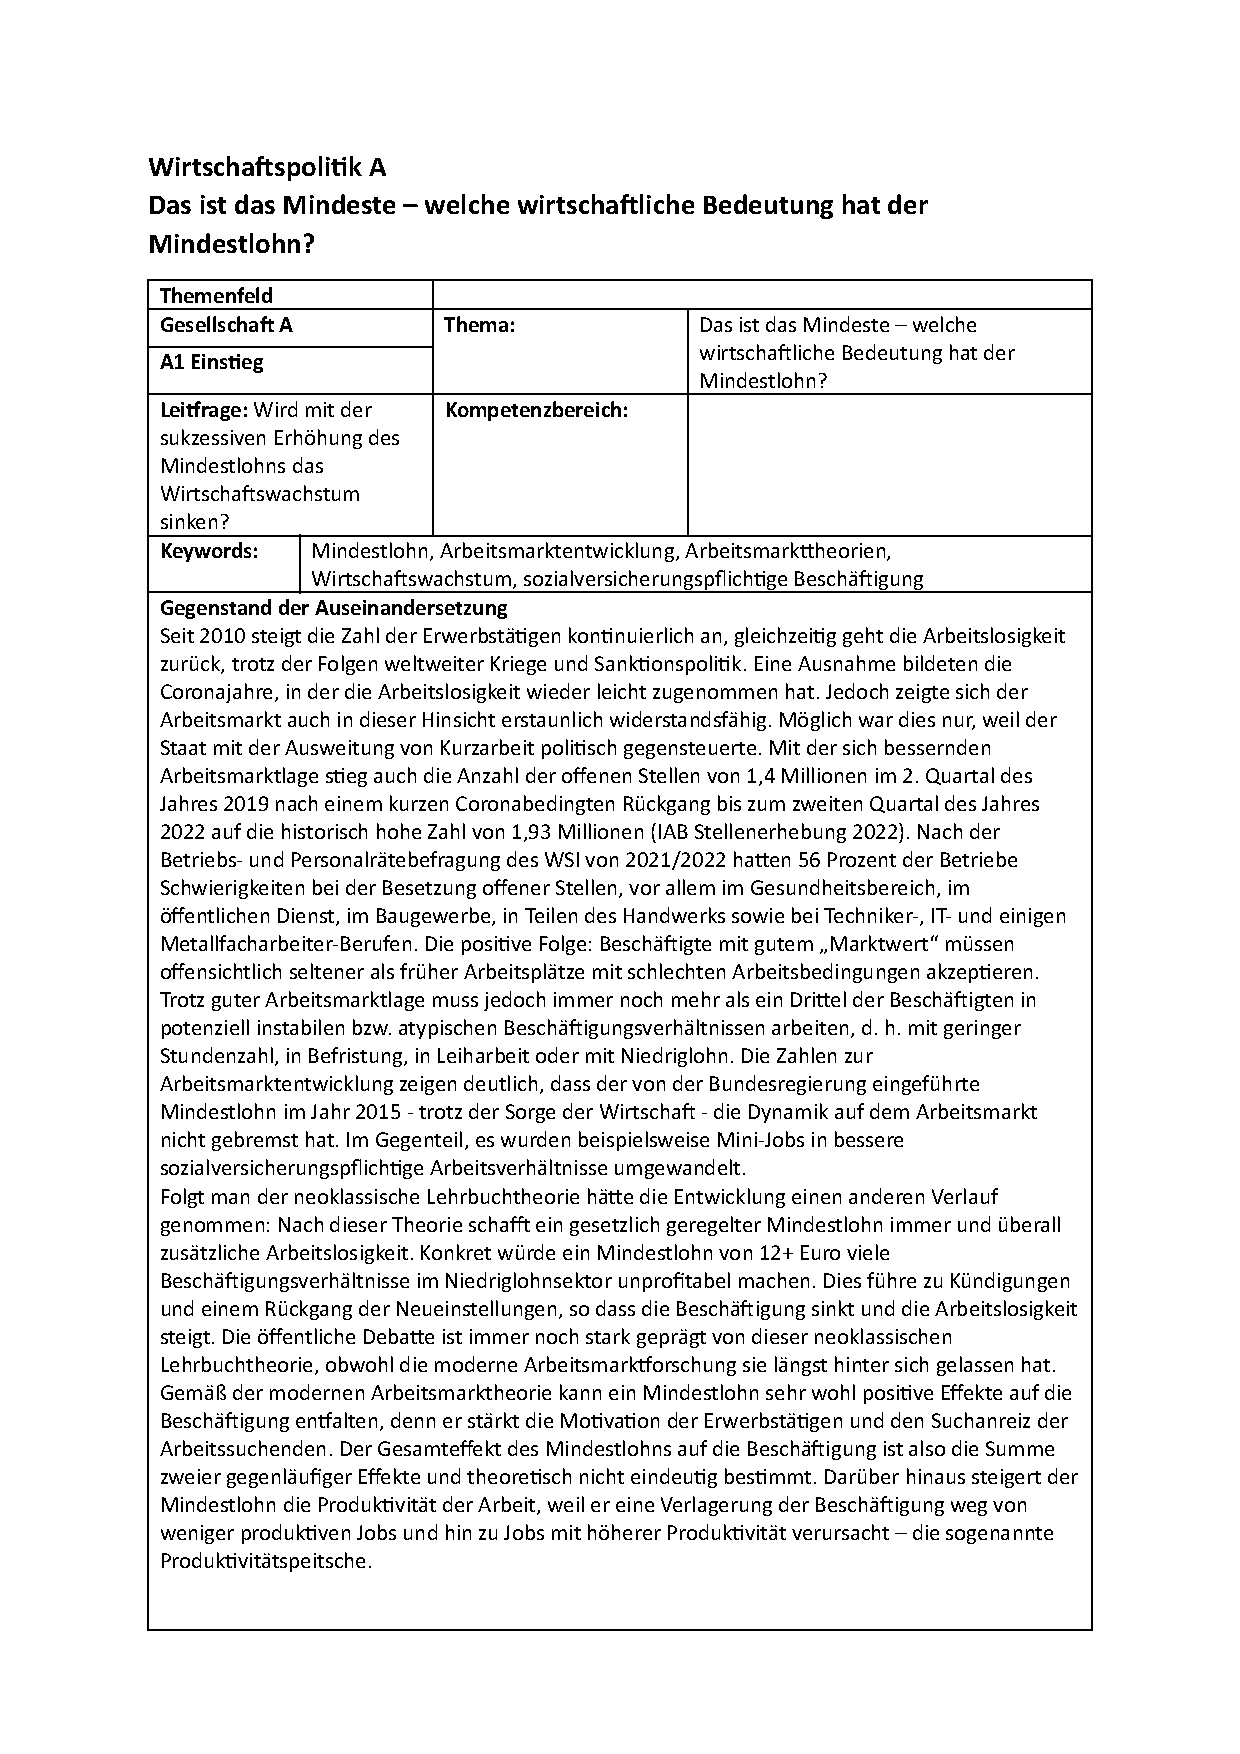
\includepdf[
    nup=2x1, 
    addtotoc={
    1, subsection, 2, Wirtschaftspolitik A1, WIRTSCHAFTSPOLITIK-A1, 
    3, subsection, 2, Wirtschaftspolitik A2, WIRTSCHAFTSPOLITIK-A2, 
    5, subsection, 2, Wirtschaftspolitik A3, WIRTSCHAFTSPOLITIK-A3, 
    7, subsection, 2, Wirtschaftspolitik B1, WIRTSCHAFTSPOLITIK-B1, 
    9, subsection, 2, Wirtschaftspolitik B2, WIRTSCHAFTSPOLITIK-B2, 
    11, subsection, 2, Wirtschaftspolitik C1, WIRTSCHAFTSPOLITIK-C1, 
    13, subsection, 2, Wirtschaftspolitik C2, WIRTSCHAFTSPOLITIK-C2
    }
]
{WIRTSCHAFTSPOLITIK.pdf}

%%%%%%%%%%%%%%%%%%%%%%%%% from page 7-8 of: https://texdoc.org/serve/pdfpages.pdf/0
% Experimental options: (Syntax may change in future versions!)
% addtotoc Adds an entry to the table of contents. This option requires five arguments, separated by commas:
% addtotoc={⟨page number⟩,⟨section⟩,⟨level⟩,⟨heading⟩,⟨label⟩}
% ⟨page number⟩: Page number of the inserted page.
% ⟨section⟩: LATEX sectioning name– e.g., section, subsection, …
% ⟨level⟩: Number, denoting depth of section– e.g., 1 for section level, 2 for
% subsection level, …
% ⟨heading⟩: Title inserted in the table of contents.
% ⟨label⟩: Name of the label. This label can be referred to with \ref and \pageref.

% Note: The order of the five arguments must not be mixed. Otherwise you will get very strange error messages.
% The addtotoc option accepts multiple sets of the above mentioned five arguments, all separated by commas. The sets must be sorted such that the ⟨page number⟩s are in ascending order. (Strictly speaking they must have the same order as the page numbers specified by the pages option.)
% The proper recursive definition of the addtotoc option is:
% addtotoc={⟨toc-list⟩}
% ⟨toc-list⟩ → ⟨page number⟩,⟨section⟩,⟨level⟩,⟨heading⟩,⟨label⟩[,⟨toc-list⟩]